\documentclass[a4paper,12pt]{report}

\usepackage[lenny,pdfpages, bclogo]{MonPaquet}
\usepackage[toc,page]{appendix}
\usepackage{amsmath,amsfonts,amssymb}
\usepackage{algorithm,algpseudocode}

\algnewcommand{\Initialize}[1]{%
  \State \textbf{Initialize:}
  \Statex \hspace*{\algorithmicindent}\parbox[t]{.8\linewidth}{\raggedright #1}
}

\begin{document}
	
\includepdf[pages={1,2,3}]{garde}	
	{\Huge{Remerciements}}

\vspace{2cm}
Nous remercions tout d'abord notre tuteur de projet \textbf{M. Yann Mathet}, enseignant-chercheur à l'université de Caen et responsable des projets de deuxième année du Master, pour ses conseils et sa disponibilité.

Merci aussi aux \textbf{administrateurs système} de l'université d'avoir été présents lorsque nous avions besoin d'eux.

Enfin, nous tenons à remercier tous \textbf{nos collègues de promotion} dans laquelle règne une atmosphère agréable de solidarité et d'entraide.


	\tableofcontents	
	{\Huge{Introduction}}

\vspace{2cm}
Ce projet prend place dans le cadre de notre Master DNR2I. Il sera fait au cours de ce rapport l'avancement de notre projet concernant le développement d'une application servant à la gestion de trajets pour les sportifs amateurs de course à pieds. Nous verrons au cours de ce rapport les enjeux du projet, nous analyserons ensuite les technologies employées ainsi que nos choix d'implémentations. Puis nous verrons en détail la réalisation du projet. Et enfin, nous terminerons par un bilan généralisant notre travail sur ce projet.	
	
	\part{Présentation et objectifs}
	\part{Présentation et objectifs}
\chapter{Présentation du projet}
\subsection{Contexte}
De nos jours, les smartphones disposent tous d'une puce GPS permettant leur géolocalisation à chaque instant avec une précision de plus en plus grande. C'est donc l'outil idéal pour les joggers et cyclistes qui souhaitent enregistrer et analyser leurs performances. De nombreuses applications ont ainsi vues le jour ces dernières années pour répondre à ces besoins. On peut notamment évoquer le leader sur le marché des applications mobiles dans la catégorie santé et remise en forme qu'est Runtastic.\\
C'est dans ce contexte que notre tuteur, M. Mathet nous a proposé de concevoir et de développer une application mobile permettant d'enregistrer les tracés GPS des parcours de l'utilisateur et d'analyser ses performances. Mais aussi, et c'est ici que tous l'enjeu du projet se situe, de comparer en temps réel les performances de l'utilisateur par rapport aux  précédentes effectuées sur le même parcours. Concrètement, il s'agit d'afficher l'avance ou le retard en secondes qu'il a par rapport à une performance définie (la meilleure ou la moyenne des dernières). 

	\chapter{Objectifs de l'application}
\section{Les trajets}
Les objectifs de ce projet sont multiples. D'abord il s'agit de réaliser une application mobile pour smartphone Android qui dispose des fonctionnalités suivantes:\bigskip

\begin{itemize}
  \item Enregistrement des coordonnées GPS du trajet
  \item Visualisation du trajet sur une carte 
  \item Consultation de l'historique des trajets 
  \item Suppression d'un trajet 
  \item Analyse des données pour obtenir :
  \begin{itemize}
    \item le temps du trajet
    \item la distance parcourue
    \item la vitesse moyenne en km/h
    \item l'allure en min/km (temps moyen pour parcourir un kilomètre)
  \end{itemize}
\end{itemize}\bigskip

\section{Les parcours}
Le second objectif est certainement le cœur du projet puisque c'est dans celui-ci que réside la nouveauté. Il s'agit de regrouper les trajets identiques pour pouvoir les comparer. Un parcours représente alors un ensemble de trajets qui suivent à peu de chose près la même trajectoire.\bigskip

Avec la mise en place de cette nouvelle structure de données nous pourrons extraire des statistiques intéressantes pour l'utilisateur à savoir:\bigskip

\begin{itemize}
  \item La meilleure performance sur le parcours
  \item Les différentes moyennes du parcours:
  \begin{itemize}
    \item le temps moyen
    \item la distance
    \item la vitesse moyenne
    \item l'allure moyenne
  \end{itemize}   
\end{itemize}\bigskip

Mais nous pourrons aussi comparer plusieurs trajectoires entre elles pour permettre à l'utilisateur de connaître en temps réel le retard ou l'avance qu'il possède par rapport à un autre trajet. L'utilisateur devra donc pouvoir fixer le trajet à prendre en référence pour chacun de ses parcours. 

\section{Le diagramme de cas d'utilisation}
A partir de ces besoins, nous avons élaboré un diagramme de cas d'utilisation qui permet de visualiser globalement le comportement de l'application. Il décrit les enchaînements d'actions que les différents acteurs peuvent effectuer. Dans notre application il n'existe qu'un seul acteur: l'utilisateur.

\begin{img}
  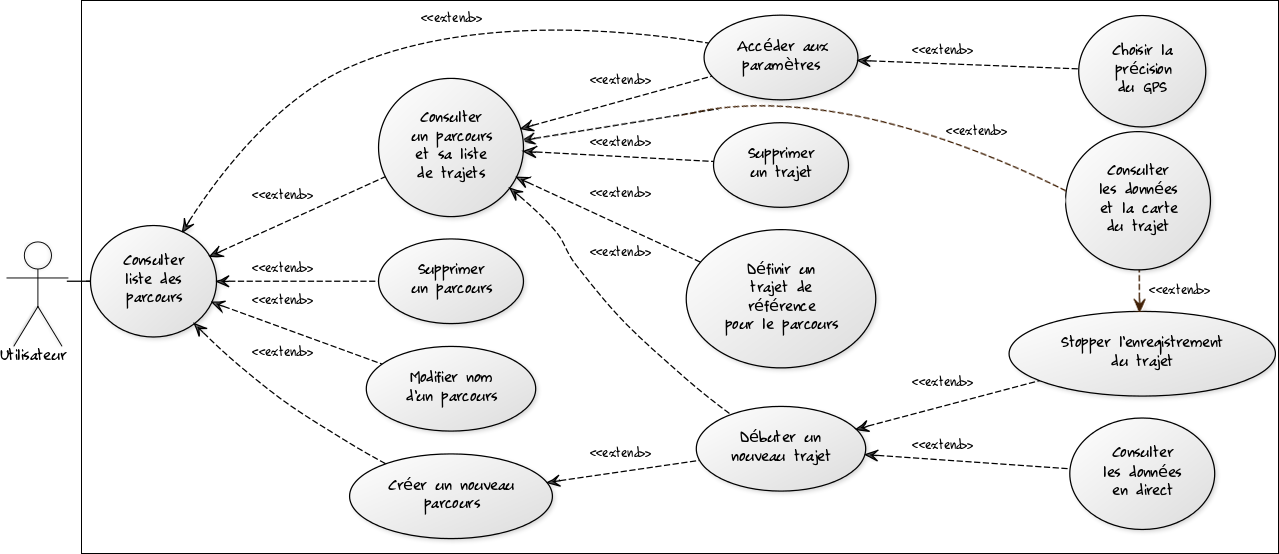
\includegraphics[scale=0.35]{img/DUC.png}
  \caption{Diagramme de cas d'utilisation de l'application}
\end{img}

\section{Les différents écrans}
Avec le diagramme de cas d'utilisation on peut facilement imaginer la structure de l'application à réaliser et le contenu des différents écrans. Quatre écrans principaux en découlent:\bigskip

\begin{itemize}
  \item La liste des parcours
  \item Le détail d'un parcours contenant sa liste de trajets
  \item Le détail d'un trajet avec l'affichage du tracé sur une carte
  \item L'écran d'enregistrement du trajet avec les données en temps réel 
\end{itemize}\bigskip

\section{Les paramètres}
On remarque un dernier cas d'utilisation nécessitant la création d'un nouvel écran, la gestion des paramètres, ou l'utilisateur pourra régler la précision du GPS. Il s'agit de définir l'intervalle d'actualisation des coordonnées GPS pour optimiser la consommation de la batterie ou la précision de son trajet. Plus la précision sera élevée, plus la consommation de la batterie sera grande et inversement.
 
	
	\part{Analyse du projet}
	\part{Analyse et implémentations}
\chapter{Détails sur l'implémentation}
\section{Représentation du modèle}
\begin{img}
  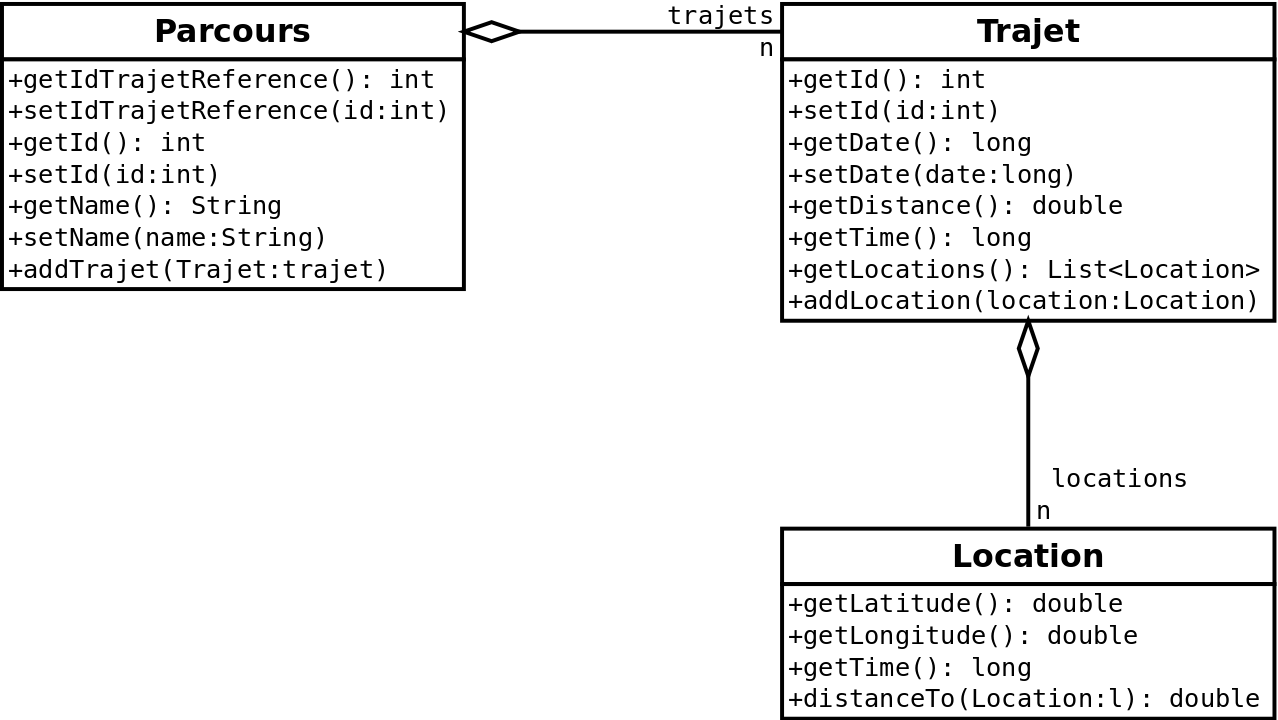
\includegraphics{img/DiagrammeDeClasse.png}
  \caption{Diagramme de classes}
\end{img}
	\chapter{Les technologies utilisées}
\section{Le choix du langage}

\subsection{Javascript}
Nous avons réalisé une étude sur les différentes technologies que nous pouvions employées pour réaliser ce projet. En effet, avec les technologies Javascript émergentes, l'utilisation de \newglossaryentry{Cordova et Phonegap}{name=Apache Cordova ou Phonegap, description={est un framework open-source développé par la Fondation Apache. Il permet de créer des applications pour différentes plates-formes (Android, Firefox OS, iOS, Ubuntu, Windows 8...) en HTML, CSS et JavaScript.}
} permettait de réaliser une application compatible avec l'ensemble des smartphones présent sur le marché actuel. Malheureusement, ces frameworks sont plutôt orientées sur des technologies web. Le développement du code avec ces technologies nécessite donc une compilation afin d'être lisible par le smartphone sur lequel il est déployé. 

\subsection{Java}
Le développement sous Android se fait dans un langage très populaire dans les systèmes embarqués, le Java. De plus, la compilation du langage est optimisée en fonction de l’appareil sur lequel il est déployé. De ce fait, l’exécution d'une application est plus performante si elle est conçue dans le langage natif au smartphone(Java pour Android, Objectif-C pour iOS). Notre application utilisant le GPS du smartphone, nous avons opté pour un développement en Java afin d'optimiser les connexions avec le satellite servant à géolocaliser le téléphone. Android étant mis à disposition par Google, il existe une documentation extrêmement fournie par l'API Google\footnote{\href{http://developer.android.com/index.html}{Google API}}

\section{Le stockage de données}
Pour un bon fonctionnement, l'application doit stocker des informations concernant les parcours et les trajets. 

\subsection{SQLite}
Sous Android (et autres smartphones), le stockage des données se fait via une base de données en SQLite. SQLite est une bibliothèque proposant un moteur de base de données relationnelles utilisant le langage SQL. Elle est plus légère que ses homologues MySQL et PostgreSQL car elle n'intègre pas le schéma habituel Client-Serveur. En effet, l'ensemble des données est stocké dans un fichier indépendant d'Android et directement intégré à l'application.

\subsection{Le format GPX}
Le GPX est un format XML conçu spécialement pour représenter un ensemble de points GPS ayant une latitude et une longitude à un instant t donné. L'utilisation de fichiers GPX est très intéressante dans notre projet dans la mesure où le GPS d'Android nous fournit des points devant d'être stockés mais sans encombrer la base. En effet, SQLite n'est pas très adapté au stockage de grosses données (big data). De plus, cette séparation permet d'extraire facilement les données liées à la représentation du trajet effectué.

\begin{xml}[Exemple de fichier GPX]
<?xml version="1.0" encoding="UTF-8" standalone="no" ?>
<gpx xmlns="http://www.topografix.com/GPX/1/1" creator="MapSource 6.9.2" version="1.1" xmlns:xsi="http://www.w3.org/2001/XMLSchema-instance" xsi:schemaLocation="http://www.topografix.com/GPX/1/1 http://www.topografix.com/GPX/1/1/gpx.xsd">
  <metadata>
    <time>2011-04-13T15:58:51Z</time>
    <bounds maxlat="49.746009" maxlon="-1.372054" minlat="49.644963" minlon="-1.925924"/>
  </metadata>
  <trk>
    <trkseg>
      <trkpt lat="49.645132" lon="-1.620045">
        <ele>-46.486572</ele>
        <time>2011-04-06T08:47:37Z</time>
      </trkpt>
     ...
      <trkpt lat="49.645703" lon="-1.619700">
        <ele>-3.227295</ele>
        <time>2011-04-06T08:49:37Z</time>
    </trkseg>
  </trk>
</gpx>
\end{xml}

\subsection{L'analyseur syntaxique}
L'utilisation de fichier GPX implique forcément un système de lecture et d'écriture de fichier XML (\textit{parser}). En Java, il existe deux grandes familles de parseurs XML, les parseurs utilisant SAX et les parseurs utilisant le DOM.

\subsubsection{Les parseurs DOM}
Les parseurs DOM analysent la structure même d'un document.Ils stockent en mémoire l'ensemble des balises XML (le DOM) afin de pouvoir retrouver n'importe quel élément du document. l'inconvénient vient du fait qu'un document ne peut pas être plus gros que la mémoire vive. 

\subsubsection{Les parseurs SAX}
Les parseurs SAX sont événementiels. En effet, ils analysent le document et déclenchent un événement lorsqu'une balise est construite ou détruite. Cette façon de lire un document est nettement moins coûteuse que la précédente dans la mesure où rien n'est stockée par le parseur. La lecture du document se fait au fur et à mesure. Cette méthode est beaucoup plus adaptée pour notre projet dans la mesure où les fichiers GPX analysés sont volumineux et les appareils n'ont pas beaucoup de mémoire. 

	\chapter{La gestion des points}

\section{La capture de points sous Android}
Sous Android, la localisation d'un appareil utilisant une puce GPS est rendue possible. Bien évidemment, plus la puce est performante plus la localisation de l’appareil sera aisée. La capture de points se fait grâce à trois fournisseurs (\textit{providers}) différents.

\subsection{Les \textit{providers}}
Nous parlerons ici uniquement des providers nécessaire au fonctionnement de notre application à savoir le \textit{NETWORK\_PROVIDER} et \textit{GPS\_PROVIDER} cependant un récapitulatif des providers est disponible à l'Annexe \ref{Annexe3}.

\subsubsection{Le \textit{NETWORK\_PROVIDER}}
Ce fournisseur détermine la position du l'appareil en fonction des antennes téléphoniques et des points d'accès au Wi-fi. Il a une précision d'environ 60 mètres. Mais fournis des points beaucoup plus rapidement que le GPS. Nous l'utilisons dans notre application le temps que la puce se synchronise avec le GPS.

\subsubsection{Le \textit{GPS\_PROVIDER}}
De tous les fournisseurs, celui-ci est de loin de plus précis puisqu'il permet de localiser un appareil avec une précision de 6 mètres. Malheureusement, pour se faire, la puce de l'appareil doit se connectée à un GPS est cela peut prendre beaucoup de temps. De plus, tant l'acquisition n'a pas été établie, aucun point ne sera fourni.

\begin{note}
L'utilisation du service de localisation sous Android nécessite des permissions que l'on doit ajouter au \textit{manifest} (Partie \ref{manifest}).
\end{note}

\subsection{Le LocationManager}
\label{locationManager}
Le \verb!LocationManager! représente le service de gestion de capture de points. C'est grâce à cette classe que la localisation de point peut se faire. Son fonctionnement est brièvement représenté par le diagramme \ref{Diagramme Location Manager}. Son instanciation se fait grâce aux services Android. Une fois l'instance obtenue, l'appel à la méthode \verb!requestLocationUpdates! doit être fait en précisant le \textit{provider} utilisé ainsi que deux variables et un \verb!LocationListener!. Les deux variables correspondent au minimum de temps et de distance nécessaire avant la capture d'un nouveau point. La valeur de ces variables est inversement proportionnelle à la consommation de la batterie. A chaque fois qu'un nouveau point est trouvé, le \verb!LocationListener!, qui écoute l'arrivée d'une nouvelle \verb!Location!, va pouvoir l'ajouter  à la liste des points du trajet. C'est également le \verb!LocationListener! qui va vérifier la bonne continuité du signal. En cas de modification, de perte ou de récupération du signal, un appel est effectué via les méthodes correspondantes.

\begin{img}  
	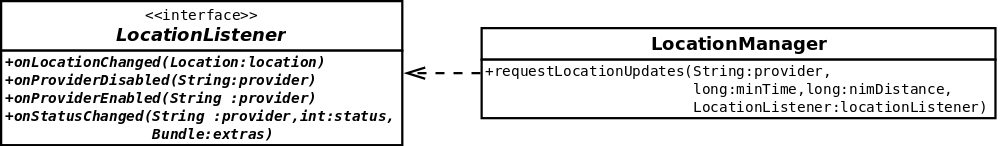
\includegraphics[scale=0.65]{img/LocationManager.png}
	\caption{Fonctionnement du Location Manager}
	\label{Diagramme Location Manager}
\end{img}

\section{Projection d'un point}
Dans la partie précédente, nous avons vu que la capture de points n'est pas très précise. En effet, pour deux trajets réalisés sur le même parcours, on peut avoir des points situés à des endroits différents et pris à des dates différentes. La figure \ref{Représentation des trajets} représente cet écart lors de la capture des points. Afin de pouvoir comparer deux trajets, nous devons projeter les points (ici le point $A$) du trajet réalisé ($t_2$) sur le trajet de référence ($t_1$). Pour cela nous devons calculer les coordonnées du point $H$ pour déterminer le rapport entre $[BH]$ et $[CH]$ et permettre une estimation sur le temps établit pour atteindre le point $A$ sur le trajet $t_1$. Nous pourrons ainsi comparer les temps mis pour atteindre les points $A$ sur $t_2$ et $H$ sur $t_1$.

\begin{img}  
	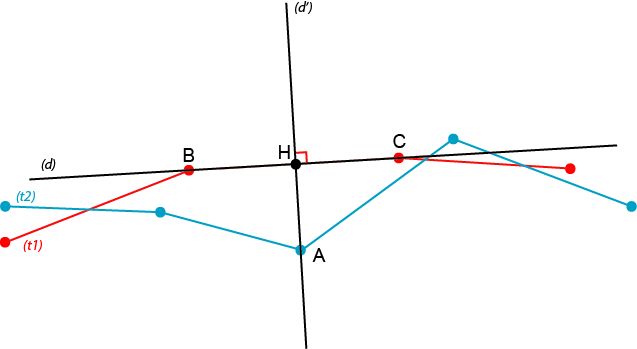
\includegraphics[scale=1]{img/Trajet.png}
	\caption{Représentation des trajets}
	\label{Représentation des trajets}
\end{img}

\subsection{Calcul des coordonnées de H}
On pose trois points $ A(x_a,y_a) $, $ B(x_b,y_b) $ et $ C(x_c,y_c) $ et nous cherchons à calculer les coordonnées de $ H(x_h,y_h) $ (Figure \ref{Représentation des trajets}).
Pour ce faire, nous devons commencer par calculer l'équation de la droite $ d $ passant par les points $B$ et $C$.
On pose donc : 
\[
 	d(x) = mx + n
\]
On cherche à déterminer le coefficient directeur de la droite ($m$). Comme $B \in d$ et $C \in d$, on a :
\[
   m =  \frac{x_b-x_c}{y_b-y_c}
\]
Comme le point $B \in (d)$, il résout l'équation :
\[
   y_b = mx_b + n \\
   \Leftrightarrow n = y_b - mx_b
\]
On cherche maintenant à déterminer l'équation de la droite $ d' $ passant par $ A $ tel que $ (d)\bot (d') $. On pose alors, 
\[
 	d'(x) = m'x + n'
\]
Comme $d$ et $d'$ sont orthogonales le produit de leur coefficient directeur est égal à 1, donc:
\[
	mm' = 1 \Leftrightarrow m' = -\frac{1}{m}	
\]
d'où
\[
	d'(x) = -\frac{1}{m}x+n'
\]
et comme $ A \in d' $, on a:
\[
	y_a = -\frac{1}{m}x_a + n' \Leftrightarrow n' = y_a + \frac{1}{m}x_a
\]
Comme $ H \in d$ et $H \in d'$, il résout le système suivant :
\begin{align}
    &\begin{cases}
   		 & y_h = -\dfrac{1}{m}x_h + n'\\
   		 & y_h = mx_h + n
    \end{cases} 
    \Leftrightarrow
    \begin{cases}
   		& x_h = -my_h + mn'\\
    	& y_h = mx_h + n
    \end{cases} 
    \Leftrightarrow
    \begin{cases}
   		& x_h = -my_h + mn'\\
    	& y_h = -y_hm^2 + m^2n' + n
    \end{cases} \\
    \Leftrightarrow
    \label{systeme}
    &\begin{cases}
   		& x_h = \dfrac{(m^2+n'+n)m}{m^2+1} + n'm \\
    	& y_h = \dfrac{(m^2+n'+n)m}{m^2+1}
    \end{cases}
\end{align}
En remplaçant les valeurs dans l'équation \eqref{systeme}, on obtient :

\begin{align}
	\begin{cases}
		 x_h = \dfrac{\left( \dfrac{x_b - x_c}{y_b - y_c}\right)^2 + y_b - \left( \dfrac{x_b - x_c}{y_b - y_c}\right) x_b + y_a + \left( \dfrac{y_b - y_c}{x_b - x_c}\right) x_a}{\left( \dfrac{x_b - x_c}{y_b - y_c}\right)^2 + 1} + \left( y_a + \left( \dfrac{y_b - y_c}{x_b - x_c}\right) x_a\right) \left( \dfrac{x_b - x_c}{y_b - y_c}\right)  \\
    	 y_h = \dfrac{\left( \dfrac{x_b - x_c}{y_b - y_c}\right)^2 + y_b - \left( \dfrac{x_b - x_c}{y_b - y_c}\right) x_b + y_a + \left( \dfrac{y_b - y_c}{x_b - x_c}\right) x_a}{\left( \dfrac{x_b - x_c}{y_b - y_c}\right)^2 + 1}
	\end{cases}
\end{align}

\subsection{Interpolation temporelle}
Après avoir récupérer les coordonnées du point $H$, nous pouvons calculer le rapport ($\theta$) entre la distance $BH$ et $HC$ et l'appliquer au temps établi pour parcourir la distance $BC$ ($\Delta_{BC}$) afin d'établir l'interpolation du temps au point $H$. Donc
\[
	t_H = \frac{distance(B,H)}{distance(B,C)}| t_B - t_C | 
\]
Nous pouvons alors comparer le temps mis pour atteindre $A$ et le temps mis pour atteindre $H$.
\begin{align}
\mbox{Si } t_H - t_A &<0 \mbox{ On est en avance.} \\
			&>0 \mbox{ On est en retard.} \\
			&=0 \mbox{ On est pareil.}
\end{align}

\section{Détermination d'un segment}
\subsection{$H \in [BC]$}
Dès lors que les coordonnées du point $H$ ont été trouvé, nous devons vérifier que $H$ appartient au segment $[BC]$. En effet, si la projection n'est pas située sur le bon segment, les résultats vont devenir incohérents. On admettra donc l'existence d'une méthode \verb!estSurSegment! permettant de vérifier que $H$ est bien compris sur le segment $[BC]$.
\subsection{L'algorithme}
Voyons maintenant l'algorithme permettant à partir d'un trajet d'établir la liste de ses points projetés sur le trajet de référence.
\begin{algorithmic}
\Function {CalculProjection}{Trajet $t_{act}$, Trajet $t_{ref}$}
\Initialize{$i_{ref} \gets 0$\\$i_{act}\gets 0$\\$projections[t_{act}.size()]$\\$H\gets null$}
\While{($i_{ref} < t_{ref}.size()-1$ and $i_{act} < t_{act}.size()$ )}
	\State $H \gets calulProjection(t_{act}[i_{act}],t_{ref}[i_{ref}],t_{ref}[i_{ref}+1])$
    \If{($estSurSegment(H, t_{ref}[i_{ref}], t_{ref}[i_{ref}+1])$)}
    	\State $projection[i_{act}]\gets H$
    	\State $i_{act}\gets i_{act}+1$
   	\Else
   		\State $i_{ref}\gets i_{ref}+1$
    \EndIf

\EndWhile
\EndFunction
\end{algorithmic}
\subsection{Les problèmes rencontrés}

	
	\part{Détail sur la réalisation}
	\chapter{Développement Android}
\section{Android en bref}
Java, activity, fragment, services, permissions

\bigskip
\begin{img}
  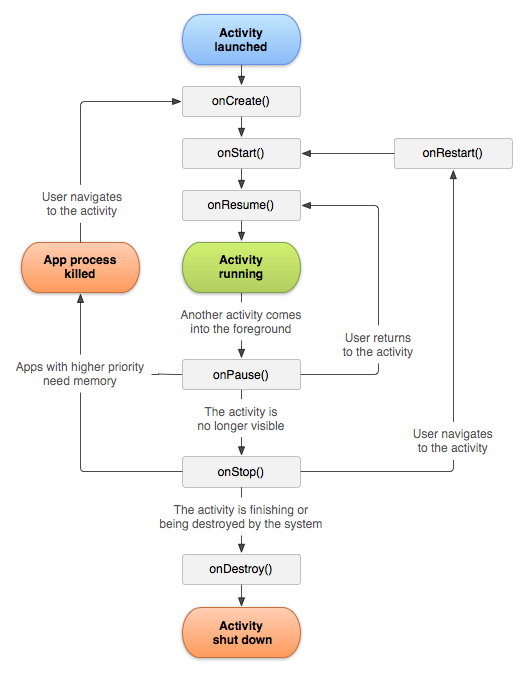
\includegraphics[scale=0.5]{img/cycle.png}
  \caption{Cycle de vie d'une Activity}
\end{img}


\section{Structure du projet}
\bigskip
\begin{multicols}{2}
\begin{img}
  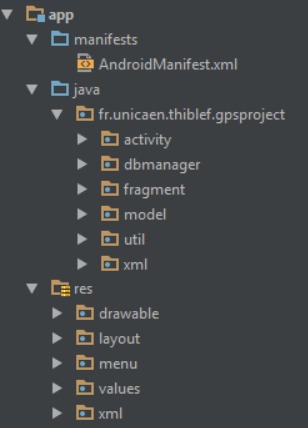
\includegraphics[scale=0.5]{img/archi.png}
  \caption{Architecture de l'application}
\end{img}

\begin{itemize}
  \item app
     \begin{itemize}
       \item manifests
       \begin{itemize}
         \item AndroidManifest.xml
       \end{itemize}
       \item java
       \begin{itemize}
         \item fr.unicaen.varlef.gpsproject
         \begin{itemize}
           \item activity
           \item dbmanager
           \item fragment
           \item model
           \item util
           \item xml
         \end{itemize}
       \end{itemize}
       \item res
       \begin{itemize}
           \item drawable
           \item layout
           \item menu
           \item values
           \item xml
         \end{itemize}
     \end{itemize}
\end{itemize}\bigskip

\end{multicols}

\section{Fonctionnement des layouts}
\begin{xml}[Exemple d'un layout]
<?xml version="1.0" encoding="utf-8"?>
<LinearLayout xmlns:android="http://schemas.android.com/apk/res/android"
    android:orientation="vertical" android:layout_width="match_parent"
    android:layout_height="match_parent">	
	<TextView
		android:id="@+id/textView"
    	android:layout_width="match_parent"
        android:layout_height="match_parent"        
        android:layout_weight="0.5"
        android:text="@string/temps" />
    <fragment
        android:id="@+id/map_container"
        android:layout_width="fill_parent"
        android:layout_height="fill_parent"
        android:layout_weight="0.5"
        class="com.google.android.gms.maps.SupportMapFragment"
        android:name="com.google.android.gms.maps.SupportMapFragment" />
</LinearLayout>
\end{xml}
\section{}



	
	\part{Bilan du projet}
	\chapter{Etat d'avancement}
\section{Fonctionnalités développées}
Au bout des ces semaines de conception et de développement nous avons une application fonctionnelle qui permet de:\bigskip

\begin{itemize}
 	\item créer, supprimer et modifier des parcours
 	\item créer, supprimer des trajets
 	\item enregistrer les coordonnées GPS du trajet 
 	\item afficher le trajet sur une carte avec son trajet de référence
 	\item définir un trajet comme référence du parcours
	\item consulter l'historique des trajets 
	\item consulter les différentes statistiques relatives aux parcours 
	\begin{itemize}
		\item la vitesse moyenne
		\item l'allure moyenne
		\item le temps moyen 
		\item les meilleurs temps et vitesse 
	\end{itemize}
 	\item consulter les différentes statistiques relatives aux trajets 
	\begin{itemize}
		\item la vitesse
		\item la distance parcourue
		\item l'allure
		\item le temps du trajet 
	\end{itemize}
\end{itemize}\bigskip

\newpage

\section{Design de l'application}
Voici à quoi ressemble l'application:\bigskip 

\begin{multicols}{2}
\begin{img}
  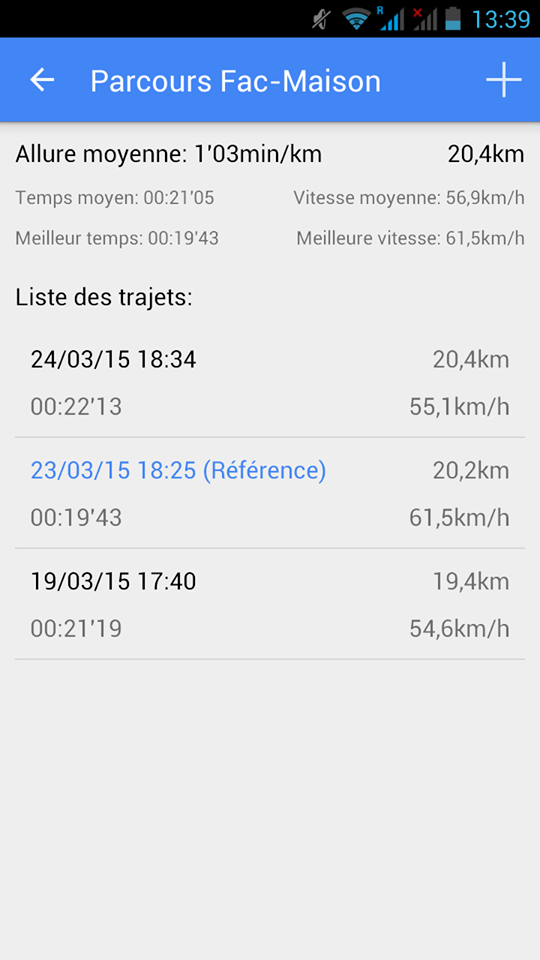
\includegraphics[scale=0.35]{img/parcours.jpg}
  \caption{Détail d'un parcours}
\end{img}
\begin{img}
  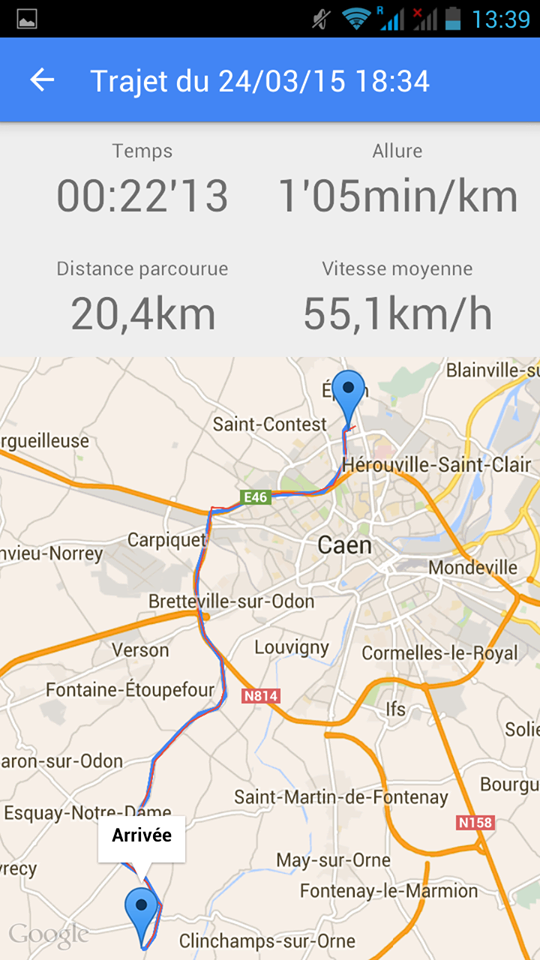
\includegraphics[scale=0.35]{img/trajet.jpg}
  \caption{Détail d'un trajet}
\end{img}
\end{multicols}

Dans l'écran de détail d'un parcours (figure 7.1) le parcours nommé "Fac-Maison" contient trois trajets triés par ordre antéchronologique. Le second parcours est défini comme trajet de référence.\bigskip

Sur la carte du détail du trajet (figure 7.2), le trajet consulté est tracé en bleu et le trajet de référence en rouge. Cela permet à l'utilisateur de déceler les éventuels écarts de parcours tout au long du trajet.
	\chapter{Les apports du projet}
\section{Les difficultés rencontrés}
Au cours de ce projet nous avons rencontré plusieurs difficultés. La première était de taille puisqu'au commencement du projet nous n'avions aucune expérience en développement Android. Même si nous avions de bonnes connaissances en Java, nous avons dû apprendre le fonctionnement des différents composants d'Android.\bigskip

La seconde difficulté réside dans l'algorithme de comparaison de deux trajets. Nous avons réussi à définir un algorithme qui traite les cas simples lorsque les deux trajectoires sont relativement proches. Mais il devient très complexe dès lors où il faut traiter tous les cas. Et même si nous n'étions pas loin de réussir, nous n'avons donc pas pu ajouter la comparaison de deux trajets en temps réel.\bigskip

Enfin, pour tester notre application nous ne disposions pas d'appareil avec une puce GPS suffisamment puissante pour capter rapidement de GPS. On se retrouvait souvent avec des acquisitions de données très hétérogènes pour un même trajet.\bigskip

\section{Apprentissage}
Au cours de ce projet, nous avons pu apprendre beaucoup de choses en matière de développement pour mobile. Les limitations apportées par la machine sont assez rares lorsque l'on développe des applications pour ordinateur. Sur mobile, même si elle est intégrée aux composants Android, la notion de développement parallèle est beaucoup plus présente que sur PC. La gestion de l'autonomie de l'appareil est également très importante et n'apparait pas du tout sur nos machines traditionnelles.
\bigskip
L'une des parties les plus intéressantes de ce projet a été de se confronter au problème de comparaison de trajets. Même si il est frustrant de ne pas avoir réussit à l'implémenter, la confrontation au problème fut très enrichissante. Il est rare à notre niveau d'avoir à ce pencher sur des problèmes qui paraissent simples mais qui sont beaucoup plus complexes.
	\chapter{Limitations et perspectives}
\section{Les limitations du produit}
Malheureusement, nous n'avons pas eu le temps de développer la totalité des fonctionnalités nécessaires pour faire de notre application un "coach" mobile. En effet la comparaison de deux trajets n'est pas terminé à cause des difficultés citées précédemment. 


\section{Les perspectives d'avenir}
Beaucoup de fonctionnalités peuvent donc être ajoutées à l'application. En mettant de côté celles citées précédemment on peut facilement imaginer beaucoup de solutions comme par exemple : \bigskip
\begin{itemize}
	\item reconnaître automatiquement si le parcours actuellement réalisé correspond à un parcours déjà effectué
	\item proposer un entrainement progressif en permettant à l'utilisateur de définir des objectifs (en temps ou en pourcentages) par rapport à un trajet précédent
	\item détecter les écarts de trajectoires
	\item synchroniser les données avec un serveur web pour permettre à l'utilisateur de consulter ses données sur le web
	\item exporter les données GPX
	\item créer des graphiques illustrant les performances de l'utilisateur
	\item calculer les calories dépensées au cours d'une courses à partir du type de course (course a pied, marche, cyclisme) et du poids de l'utilisateur
\end{itemize}


	{\Huge{Conclusion}}

\vspace{2cm}

	{\Huge{Glossaire}}

\vspace{2.5cm}

{\bfseries Apache Cordova ou Phonegap:} est un framework open-source développé par la Fondation Apache. Il permet de créer des applications pour différentes plates-formes (Android, Firefox OS, iOS, Ubuntu, Windows 8...) en HTML, CSS et JavaScript.
\bigskip

{\bfseries Base de données:} c’est un ensemble de données stockées qui peuvent être accédées et modifiées via un langage de manipulation de données.
\bigskip

{\bfseries Bibliothèque / Librairie:} désigne un groupe de fonctionnalités dont les caractéristiques sont éditées, et donc à la disposition de différentes applications.
\bigskip

{\bfseries JavaScript:} c’est un langage de programmation orienté objet, principalement utilisé dans les pages web.
\bigskip

{\bfseries Modélisation:} Action de décrire un système réel de façon formelle, de façon à pouvoir le manipuler par ordinateur.
\bigskip

{\bfseries SAX (Simple API for XML):} API basée sur un mode événementiel permettant de réagir à des événements (comme le début d'un élément, la fin d'un élément) et de renvoyer le résultat à l'application.
\bigskip



	{\Huge{Sources}}

\vspace{2cm}	
	\newpage
	\appendix
	\begin{appendices}
\chapter{L'ajout de points}

\label{Annexe1}
\begin{java}[L'ajout de point à un trajet]  
public void addLocation(Location l) {
	//Si il n'y a pas de points d'enregistres
	if (locations.size() == 0) {
		distance = 0;
		locations.add(l);
		temps = 0;
	} else {
	
	//On recupere la derniere position 
	Location last = getLastPosition();
	
	//On augmente la distance total du trajet 
	distance += last.distanceTo(l);
	locations.add(l);
 	
 	//On incremente egalement le temps 
	if (locations.size() == 1) {
		temps = 0;
	} 
	temps += ((l.getTime() / 1000) - (last.getTime() / 1000));   
	}
}
\end{java}

\chapter{Calcul de la distance entre deux points géolocalisés}
\label{Annexe2}

\chapter{Les providers Android}
\label{Annexe3}
\begin{center}
   \begin{tabular}{| c | c | l | }
     \hline
     Accuracy & Power Usage & Technology \\ \hline
     20ft & High & Autonomous GPS, Provider: gps \\ 
     && uses GPS chip on the device \\
     && line of sight to the satellites \\
     && need about 7 to get a fix \\
     && takes a long time to get a fix \\
     && doesn’t work around tall buildings \\ \hline
 
     200ft & Medium & Assisted GPS (AGPS), Provider: network \\ 
     && uses GPS chip on device \\
	 && very low power consumption \\
	 && very accurate \\
	 && works without any line of sight to the sky \\
	 && depends on carrier and phone supporting this \\ \hline
    
    1 mile & Low & CellID lookup/WiFi MACID lookup, Provider: network or passive \\
     && very fast lock, and does not require GPS chip on device to be active \\
	 && requires no extra power at all \\ 
     && has very low accuracy \\
     \hline
   \end{tabular}
 \end{center}
\caption{Les providers Android\footnote{\href{http://developerlife.com/tutorials/?p=1375}{Source}}}

\chapter{Captures d'écrans de l'application}
\label{Annexe3}
\begin{multicols}{3}
\begin{img}
  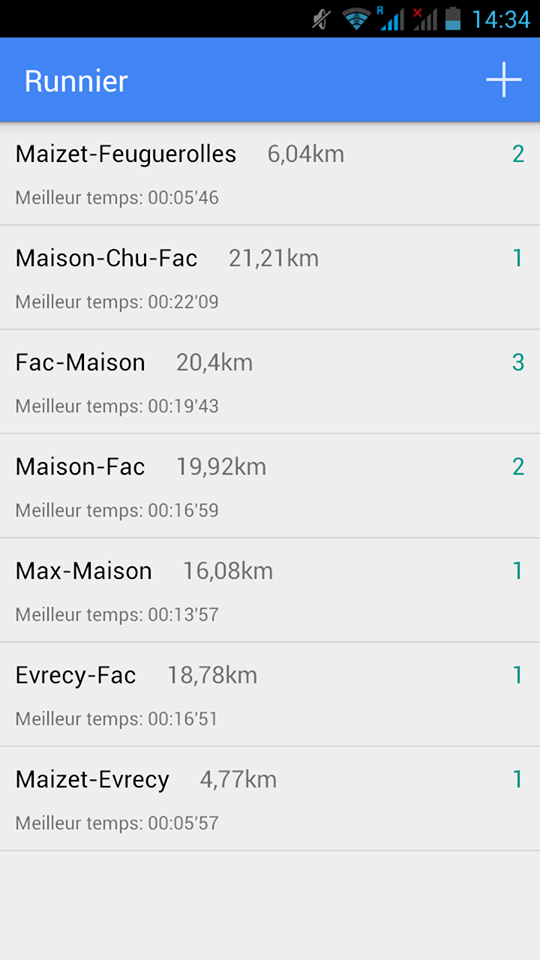
\includegraphics[scale=0.3]{img/home.jpg}
  \caption{Liste des parcours}
\end{img}
\begin{img}
  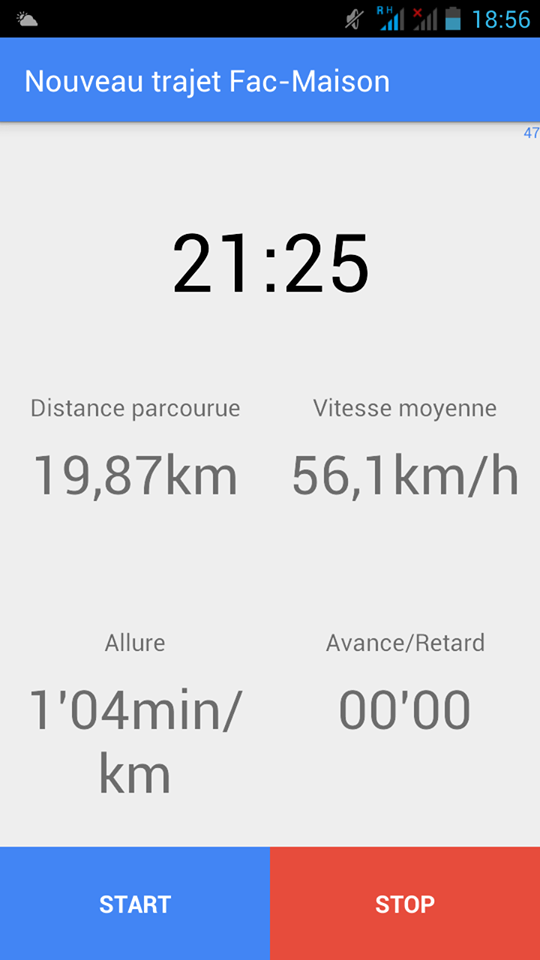
\includegraphics[scale=0.3]{img/direct.jpg}
  \caption{Enregistrement d'un trajet}
\end{img}
\begin{img}
  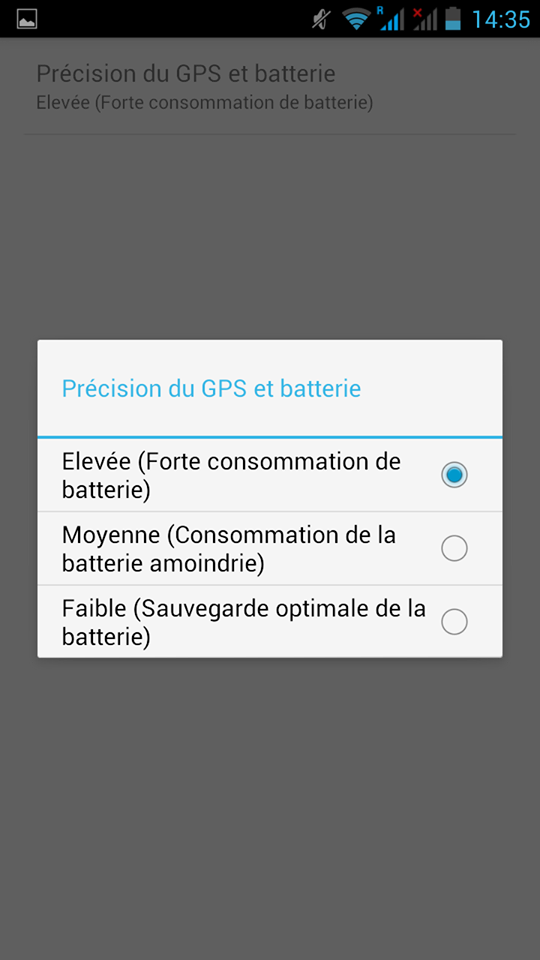
\includegraphics[scale=0.3]{img/parametres.jpg}
  \caption{Paramètres}
\end{img}
\end{multicols}

\end{appendices}



	
\includepdf{resume}
\end{document}


